\chapter{Kurzanalyse}
\label{chapter-analyse}

Für die Entwicklung eines Dating-Protokolls ist es zwingend notwendig, eine Analyse der geistig verwirrten Hobby-Coaches durchzuführen.
Dabei soll verstanden werden, was der arme Timmy in den nächsten Stunden seines Dating-Coaching durchmachen muss und welche groben Fehler seitens der Coaches begangen werden.
Wer an dieser Stelle einen Methodik-Teil erwartet haben, wird diese nicht bekommen.
Schließlich muss sich auf das subjektive Niveau der Youtuber begeben werden, um diese auch analysieren zu können.

\section{Blub}


\begin{figure}
    \centering
    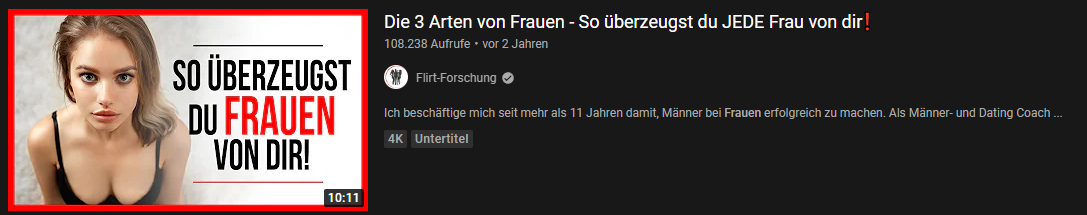
\includegraphics[scale=0.4]{Sources/clickbait.png}
    \caption{TODO: Link: \url{https://www.youtube.com/watch?v=gr3fFu3vVCM}}
    \label{fig:analyse-clickbait}
\end{figure}